\documentclass[10pt]{article}
\usepackage[spanish]{babel}
\usepackage{graphicx}
\usepackage{amssymb}
\usepackage{epstopdf}
\usepackage{enumitem}
\usepackage{multicol,multirow}
\DeclareGraphicsRule{.tif}{png}{.png}{`convert #1 `dirname #1`/`basename #1 .tif`.png}

% For a visual definition of these parameters, see
\textwidth = 6.5 in
\textheight = 9 in
\oddsidemargin = 0.0 in
\evensidemargin = 0.0 in
\topmargin = 0.0 in             
\headheight = 0.0 in            
\headsep = 0.0 in
            
\parskip = 0.2in                % vertical space between paragraphs
% Delete the % in the following line if you don't want to have the first line of every paragraph indented
%\parindent = 0.0in

\begin{document}
    \begin{center}
        {\Large Pauta Certamen 2, Programaci\'on II} \\
        \emph{\small Prof. Rodrigo Olivares} \\
    \end{center}
    \vspace*{-35pt}
    \begin{center}
        \rule{1\textwidth}{.3pt}
    \end{center}
    \vspace*{-42pt}
    \begin{center}
        \rule{1\textwidth}{2pt}
    \end{center}

    \vspace*{-15pt}
    {\small \textbf{Instrucciones}:}
    \vspace*{-15pt}

    {\scriptsize
    \begin{itemize}
        \item[-] El puntaje m\'aximo del certamen es 100\%, siendo el 60\% el m\'inimo requerido para aprobar.
        \item[-] Responda las preguntas en un \'unico archivo, agregando el n\'umero de la pregunta, su nombre y RUT. Si no responde alguna pregunta, debe indicar en el mismo archivo que \textbf{no responde}. El nombre del archivo debe tener la forma $<<$\emph{apellido\_nombre.ext}$>>$ y debe ser subido al aula virtual.
        \item[-] El certamen es \underline{\textbf{individual}}. Cualquier intento de copia, ser\'a sancionado con nota \textbf{1,0}.
    \end{itemize}
    
    \vspace*{-25pt}

    \begin{enumerate}

        \item \emph{30pts (6pts c/u).} \textbf{Comente} las siguientes declaraciones.
    
        \begin{enumerate}[label=(\alph*)]
            \item La herencia es un mecanismo que permite construir clases tipo Padre-Hija(s). Esta construcci\'on es llevada a cabo sin la necesidad de conocer el comportamiento de la clase Padre.
            \item[\textbf{R:}] Es \textbf{cierto} que la herencia es un mecanismo que permite construir clases tipo Padre-Hija(s), sin embargo esta construcci\'on debe ser llevada a cabo conociendo el comportamiento de la clase Padre, pues es de vital importancia saber \textbf{qu\'e} hace la clase Padre sin importar el \textbf{c\'omo}.
            \item En la implementaci\'on de una clase abstracta, la sub-clase que la extiende debe manipular todos los m\'etodos, sean o no abstractos.
            \item[\textbf{R:}] La sub-clase que extiende a una clase abstracta no est\'a obligada a implementar los m\'etodos abstractos, sin embargo se deben re-definir nuevamente como \textbf{abstract}. Para los m\'etodos no \textbf{abstract}, no existe obligaci\'on de re-definirlos.
            \item La el uso de interfaces permite simular la herencia m\'ultiple. 
            \item[\textbf{R:}] Ciertamente la herencia m\'ultiple no existe en Java, sin embargo \'esta puede ser simulada a partir de la implementaci\'on de diversas interfaces.
            \item Una lista es un tipo de dato abstracto gen\'erico, ideal para gestionar colecciones de datos.
            \item[\textbf{R:}] Una lista es una interfaz que puede ser implementada por diversas clases. Es cierto que una lista puede ser un TDA y el comportamiento estar\'a definido por la implentaci\'on (clase que la implementa).
            \item La entidad es un compomente fundamental en la programaci\'on orientada a objeto.
            \item[\textbf{R:}] Una entidad es un tipo de dato abstracto (TDA) definida por el programador (clase) y cumple un rol fundamental en la programación orientada a objeto (permite realizar instancias/objetos). Estas entidades permiten matear un concepto de la vida real a una entidad l\'ogica de programaci\'on. Esta entidad es indivisible (entidad at\'omica).
        \end{enumerate}
\newpage
        \item \emph{70pts.} Considere 3 dataset: \emph{regiones.txt}, \emph{provincias.txt} y \emph{comunas.txt}: La informaci\'on contenida es la siguiente:
        \begin{enumerate}
            \item[-] \emph{regiones.txt}: identificador y nombre de la regi\'on.
            \item[-] \emph{provincias.txt}: identificador y nombre de la provincia, adem\'as del identificador de la regi\'on a la que pertenece.
            \item[-] \emph{comunas.txt}: identificador y nombre de la comuna, adem\'as del identificador de la provincia a la que pertenece.
            \item[] De acuerdo a esto, debe:
        \begin{enumerate}
            \item[\emph{20pts}] Construir las entidades que permitan mapear los dataset. Utilice \textbf{herencia} para ''heredar'' el compartamiento com\'un (ver figura \ref{fig:diagrama}).
            \item[\emph{40pts}] Construya un clase que:
            \begin{enumerate}[label=(\alph*)]
                \item[\emph{30pts}] Desarrolle los m\'etodos de lectura de los dataset.
                \item[\emph{10pts}] Desarrolle los m\'etodos necesarios para ''buscar'' la informaci\'on en las listas de objetos.
            \end{enumerate}
            \item[\emph{10pts}] Construya la clase y el m\'etodo principal para la ejecuci\'on del programa.
        \end{enumerate}
         \end{enumerate}
    \end{enumerate}

    \begin{figure}[htbp!]
        \begin{center}
            \fbox{\fbox{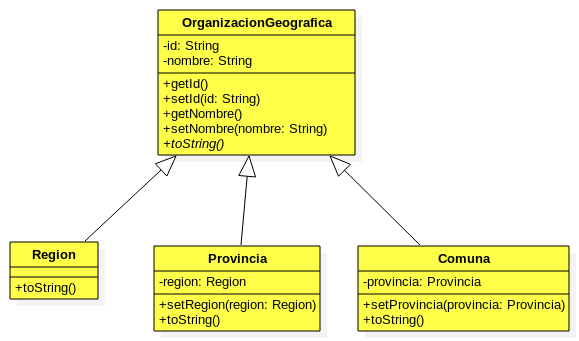
\includegraphics[scale=.5]{images/diagrama.png}}}
            \caption{{\scriptsize Diagrama de clase/entidades}}\label{fig:diagrama}
        \end{center}    
    \end{figure}
    \textbf{**Revisar archivos java adjuntos.}
        \newpage
    Para la pregunta \emph{2.-}, considere el uso de la siguiente clase:
        \begin{multicols}{2}
            \begin{verbatim}
import java.io.BufferedReader;
import java.io.File;
import java.io.FileReader;
import java.io.FileWriter;
import java.io.IOException;
import java.io.PrintWriter;
import java.util.ArrayList;
import java.util.List;

public class LecturaEscritura {

    public List<String> leer(String nombreArchivo) {

        File archivo;
        FileReader fr = null;
        List<String> lineas = null;

        try {
            archivo = new File(nombreArchivo);
            lineas = new ArrayList<String>();
            String linea;
            fr = new FileReader(archivo);
            BufferedReader br = new BufferedReader(fr);

            while ((linea = br.readLine()) != null) {
                lineas.add(linea);
            }
        } catch (IOException e) {
            System.out.println(e);
        } finally {
            try {
                if (fileReader != null) {
                    fileReader.close();
                }
            } catch (IOException e) {
                System.out.println(e);
            }
        }
        return lineas;
    }

    public void escribir(String nombreArchivo, 
                         List<String> lineas) {

        FileWriter archivo;
        PrintWriter printWriter = null;

        try {
            archivo = new FileWriter(nombreArchivo, true);
            printWriter = new PrintWriter(archivo);

            for (String linea : lineas) {
                printWriter.println(linea);
            }
        } catch (IOException e) {
            System.out.println(e);
        } finally {
            printWriter.close();
        }
    }
}
            \end{verbatim}
        \end{multicols}
        \vspace*{-20pt}
        \begin{center}
            \textbf{\textquestiondown C\'omo ser\'e evaluado en la pregunta 1?} \linebreak
            \begin{tabular}{|p{2cm}|p{4cm}|p{4cm}|p{4cm}|}\hline
                \multicolumn{1}{|c|}{\textbf{T\'opico}} & 
                \multicolumn{1}{c|}{\textbf{Logrado}} & 
                \multicolumn{1}{c|}{\textbf{Medianamente logrado}} & 
                \multicolumn{1}{c|}{\textbf{No logrado}} \\ \hline
                Herencia & 
                \emph{6pts} Comenta satisfactoriamente el mecanismo de herencia en la relaci\'on \textbf{es-un}. & 
                \emph{3pts} Comenta parcialmente el mecanismo de herencia en la relaci\'on \textbf{es-un}, dejando dudas respecto a la jerarqu\'ia Padre-Hijo. & 
                \emph{1pts} Comenta err\'oneamente el mecanismo de herencia en la relacion \textbf{es-un}.\\ \hline
                Clase abstracta & 
                \emph{6pts} Comenta satisfactoriamente el concepto de clase abstracta. & 
                \emph{3pts} Comenta parcialmente el concepto de clase abstracta, dejando dudas respecto a la manipulaci\'on de sus m\'etodos. & 
                \emph{1pts} Comenta err\'oneamente el concepto de clase abstracta.\\ \hline
                Interfaces & 
                \emph{6pts} Comenta satisfactoriamente la ''simulaci\'on'' de herencia m\'ultiple. & 
                \emph{3pts} Comenta parcialmente la herencia m\'ultiple, no utilizando interfaces. & 
                \emph{1pts} Comenta err\'oneamente la ''simulaci\'on'' de herencia m\'ultiple. \\ \hline
                TDA Lista & 
                \emph{6pts} Comenta satisfactoriamente el uso de TDA Listas para la colecci\'on de objetos. & 
                \emph{3pts} Comenta parcialmente el uso de TDA Listas para la colecci\'on de objetos, dejando dudas respecto a la manipulaci\'on de \'estos. & 
                \emph{1pts} Comenta err\'oneamente el uso de TDA Listas. \\ \hline
                TDA Bean & 
                \emph{6pts} Comenta satisfactoriamente el uso de TDA Beans como principal componente de la POO. & 
                \emph{3pts} Comenta parcialmente el uso de TDA Beans como principal componente de la POO, dejando dudas respecto a la utilidad de \'estos. & 
                \emph{1pts}  Comenta err\'oneamente el uso de TDA Beans. \\ \hline
                Total m\'aximo puntaje pregunta 1 & 
                \emph{30pts} & 
                \emph{15pts} & 
                \emph{5pts} \\ \hline
            \end{tabular}
        \end{center}
        \vspace*{-20pt}
        \begin{center}
            \textbf{\textquestiondown C\'omo ser\'e evaluado en la pregunta 2?} \linebreak
            \begin{tabular}{|p{2cm}|p{4cm}|p{4cm}|p{4cm}|}\hline
                \multicolumn{1}{|c|}{\textbf{T\'opico}} & 
                \multicolumn{1}{c|}{\textbf{Logrado}} & 
                \multicolumn{1}{c|}{\textbf{Medianamente logrado}} & 
                \multicolumn{1}{c|}{\textbf{No logrado}} \\ \hline
                Construir entidades & 
                \emph{20pts} Aplica en forma correcta la herencia con el desarrollo de las entidades. & 
                \emph{12pts} No aplica de forma correcta la herencia, pero si construye las entidades. & 
                \emph{6pts} No aplica de forma correcta la herencia y no construye las entidades. \\ \hline
                Construir clase UbicacionImpl & 
                \emph{40pts} Construye satisfactoriamente la clase e implementa todos los m\'etodos de lectura de los dataset y b\'usqueda de informaci\'on en las listas de objetos. & 
                \emph{25pts} Construye la clase con lectura parcial de los dataset, con s\'olo algunos m\'etodos de b\'usqueda de informaci\'on en las listas de objetos. & 
                \emph{12pts} No construye la clase. \\ \hline
                Construir clase principal & 
                \emph{10pts} Construye satisfactoriamente la clase principal y el m\'etodo est\'atico main, con las instancias de los objetos y la llamada a sus m\'etodos. & 
                \emph{5pts} Construye la clase principal con el m\'etodo est\'atico main, pero no realiza correctamente las instancias de los objetos y las llamadas a los m\'etodos. & 
                \emph{0pts} No construye la clase principal. \\ \hline
                Total m\'aximo puntaje pregunta 2 & 
                \emph{70pts} & 
                \emph{42pts} & 
                \emph{18pts} \\ \hline
            \end{tabular}
        \end{center}

    }
\end{document} 
